\section{Data Preparation}

We also looked at the outliers we already detected with the box plots in the previous section.\\
As we can see in Figure \ref{fig:sale_qta_boxplots_after}, the previous operations already cleaned some of the outliers we had in the original dataset; now we manually check them, to determine if they are errors or not.

In the case of \emph{Sale}, we have that the maximum value is 649.5, which is quite high but we discovered that this purchase is referred to a 60 pieces of an item, \emph{i.e. picnic basket wicker 60 pices}, so we proceed by dividing the \emph{Sale} value by 60 and incrementing the \emph{Qta} with the same value.\\
In the case of \emph{Qta}, we see just one value are really away from the others, and it represent huge purchases, with quantity equal to 12540. We consider this row as correct.

\begin{figure}[h!]
\captionsetup{justification=centering}
\begin{subfigure}{.3\textwidth}
\centering
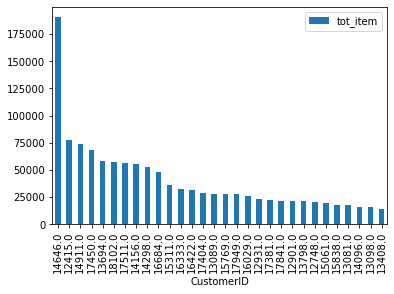
\includegraphics[width=\textwidth]{img/tot_item.png}
\caption{Total number of items per customer}
\label{fig:tot_item}
\end{subfigure}
\begin{subfigure}{.3\textwidth}
\centering
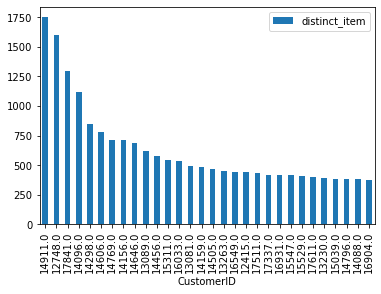
\includegraphics[width=\textwidth]{img/distinct_item.png}
\caption{Number of distinct items per customer}
\label{ref:distinct_item}
\end{subfigure}
\begin{subfigure}{.3\textwidth}
\centering
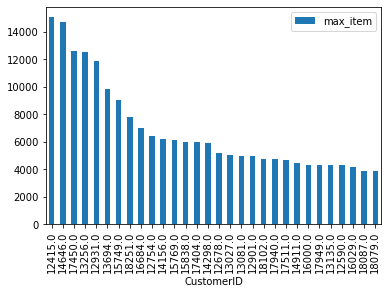
\includegraphics[width=\textwidth]{img/max_item.png}
\caption{Maximum number of items per customer}
\label{fig:max_item}
\end{subfigure}
\caption{Visualization for the extracted features}
\label{fig:first_features}
\end{figure}

At this point, in order to describe the customers behavior, we extract the following new features from the dataset:\\
First of all, we defined some basic features, like:
\begin{itemize}
\item The total number of items purchased by a customer
\item The number of distinct items bought by a customer
\item The maximum number of items purchased by a customer during a shopping session
\end{itemize}

In Figure \ref{fig:first_features}, we can see some visualization for these features; in particular, they represent the first 30 customers with the biggest values for each feature.\\
An interesting information is clear from the plot \ref{fig:max_item}, where we can see that the maximum quantities purchased in a single shopping session are very big; they are all above 3500, with the maximum equal to 15049. These are very high values, unlikely for a retail customer; this led us to think that the supermarket in question also sells wholesale.

In Figure \ref{fig:kde_entropy}, we can evaluate the distribution of the entropy. In particular, we are focusing on the attribute \emph{TotSale}.
This value of the entropy represents the variability of the customer's spending habits; a bigger value means that the customer did not have a regular behavior, instead he spent always different amount of money.\\
We have a small peak corresponding to 0, meaning that there are some customers with very specific habits, but the maximum is reached for $\sim 4$, which means that the majority of the clients have a quite unpredictable behavior.

Since the focus is on the purchasing behavior of the customers, we decided to study other features, in order to deeply understand the information we have. We chose to extract information about:
\begin{itemize}
\item The number of basket per customer
\item The number of \emph{bad} basket per customer
\item The number of purchased products
\item The number of returned products
\item The amount of money spent for each customer
\item The amount of money refunded per customer
\end{itemize}

Thanks to these features, we were able to outline better the kind of customers registered in the dataset.\\
First, we checked if there were customers with a number of returned products bigger than the purchased ones; as a matter of fact, we found \textbf{18} rows of this kind. We consider these as \emph{bad} customers, since they have made more returns than purchases; this is clearly an impossible situation, maybe due to the fact that some transaction was not registered in the dataset.
Anyway, we decided to delete these customers.\\
Plus, we inserted two other columns:
\begin{itemize}
\item \textbf{ActualQta}, which is the algebraic sum between the positive and the negative quantities
\item \textbf{ActualSpent}, equal to the difference between the money spent and the one refunded
\end{itemize}

We also deleted all the customers with the \textbf{ActualQta} equal to zero, since, in the end, they didn't buy anything. 

Now we extract some information about the average values, as:
\begin{itemize}
\item \textbf{AvgPrice}, the ratio between \textbf{ActualSpent} and \textbf{ActualQta}, that represents the average price of the products bought by a customer
\item \textbf{AvgBaskValue}, the ratio between \textbf{ActualSpent} and the number of \emph{good} baskets, which represents the average amount of money spent for each basket per customer
\end{itemize}

Another interesting feature is the \textbf{MonthFreq}, that we computed as the ratio between the number of \emph{good} baskets and 12, the number of months. We can visualize this attribute in Figure \ref{fig:month_freq}, where we can clearly see that the peak is really close to 0; in fact, the mode of this column in equal to \textbf{0.083}, which means that the majority of the customers went to this supermarket just once in the year.

\begin{figure}
\captionsetup{justification=centering}
\begin{subfigure}{0.49\textwidth}
\centering
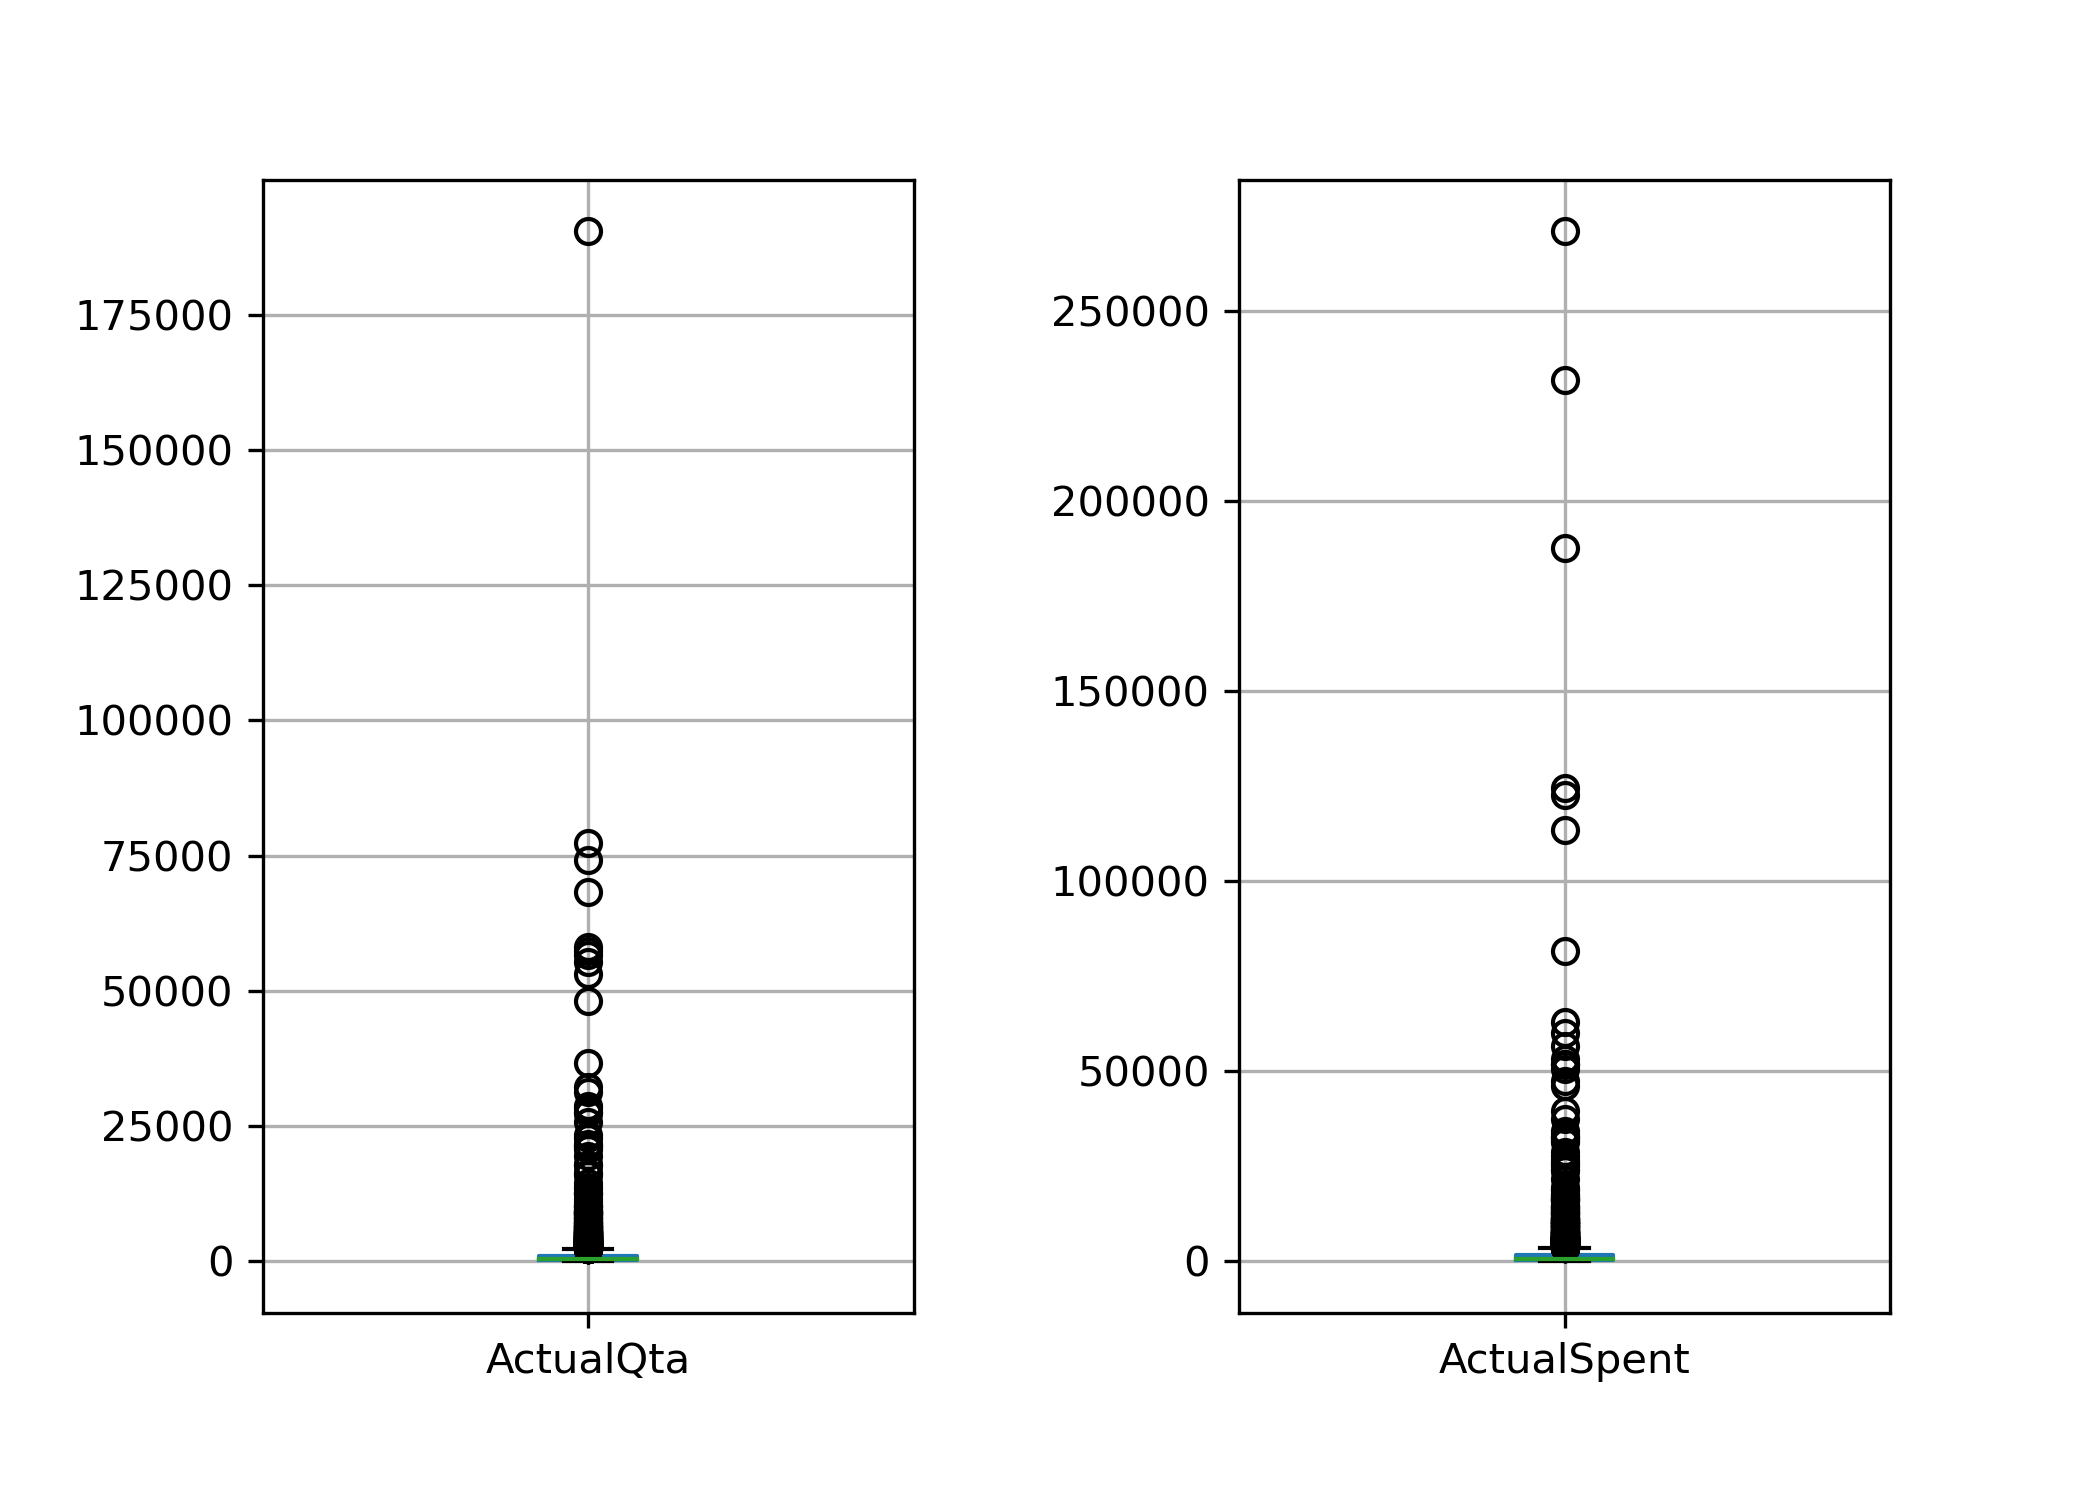
\includegraphics[width=\textwidth]{img/boxplot_for_actuals.png}
\caption{}
\label{fig:boxplot_actuals}
\end{subfigure}
\begin{subfigure}{0.49\textwidth}
\centering
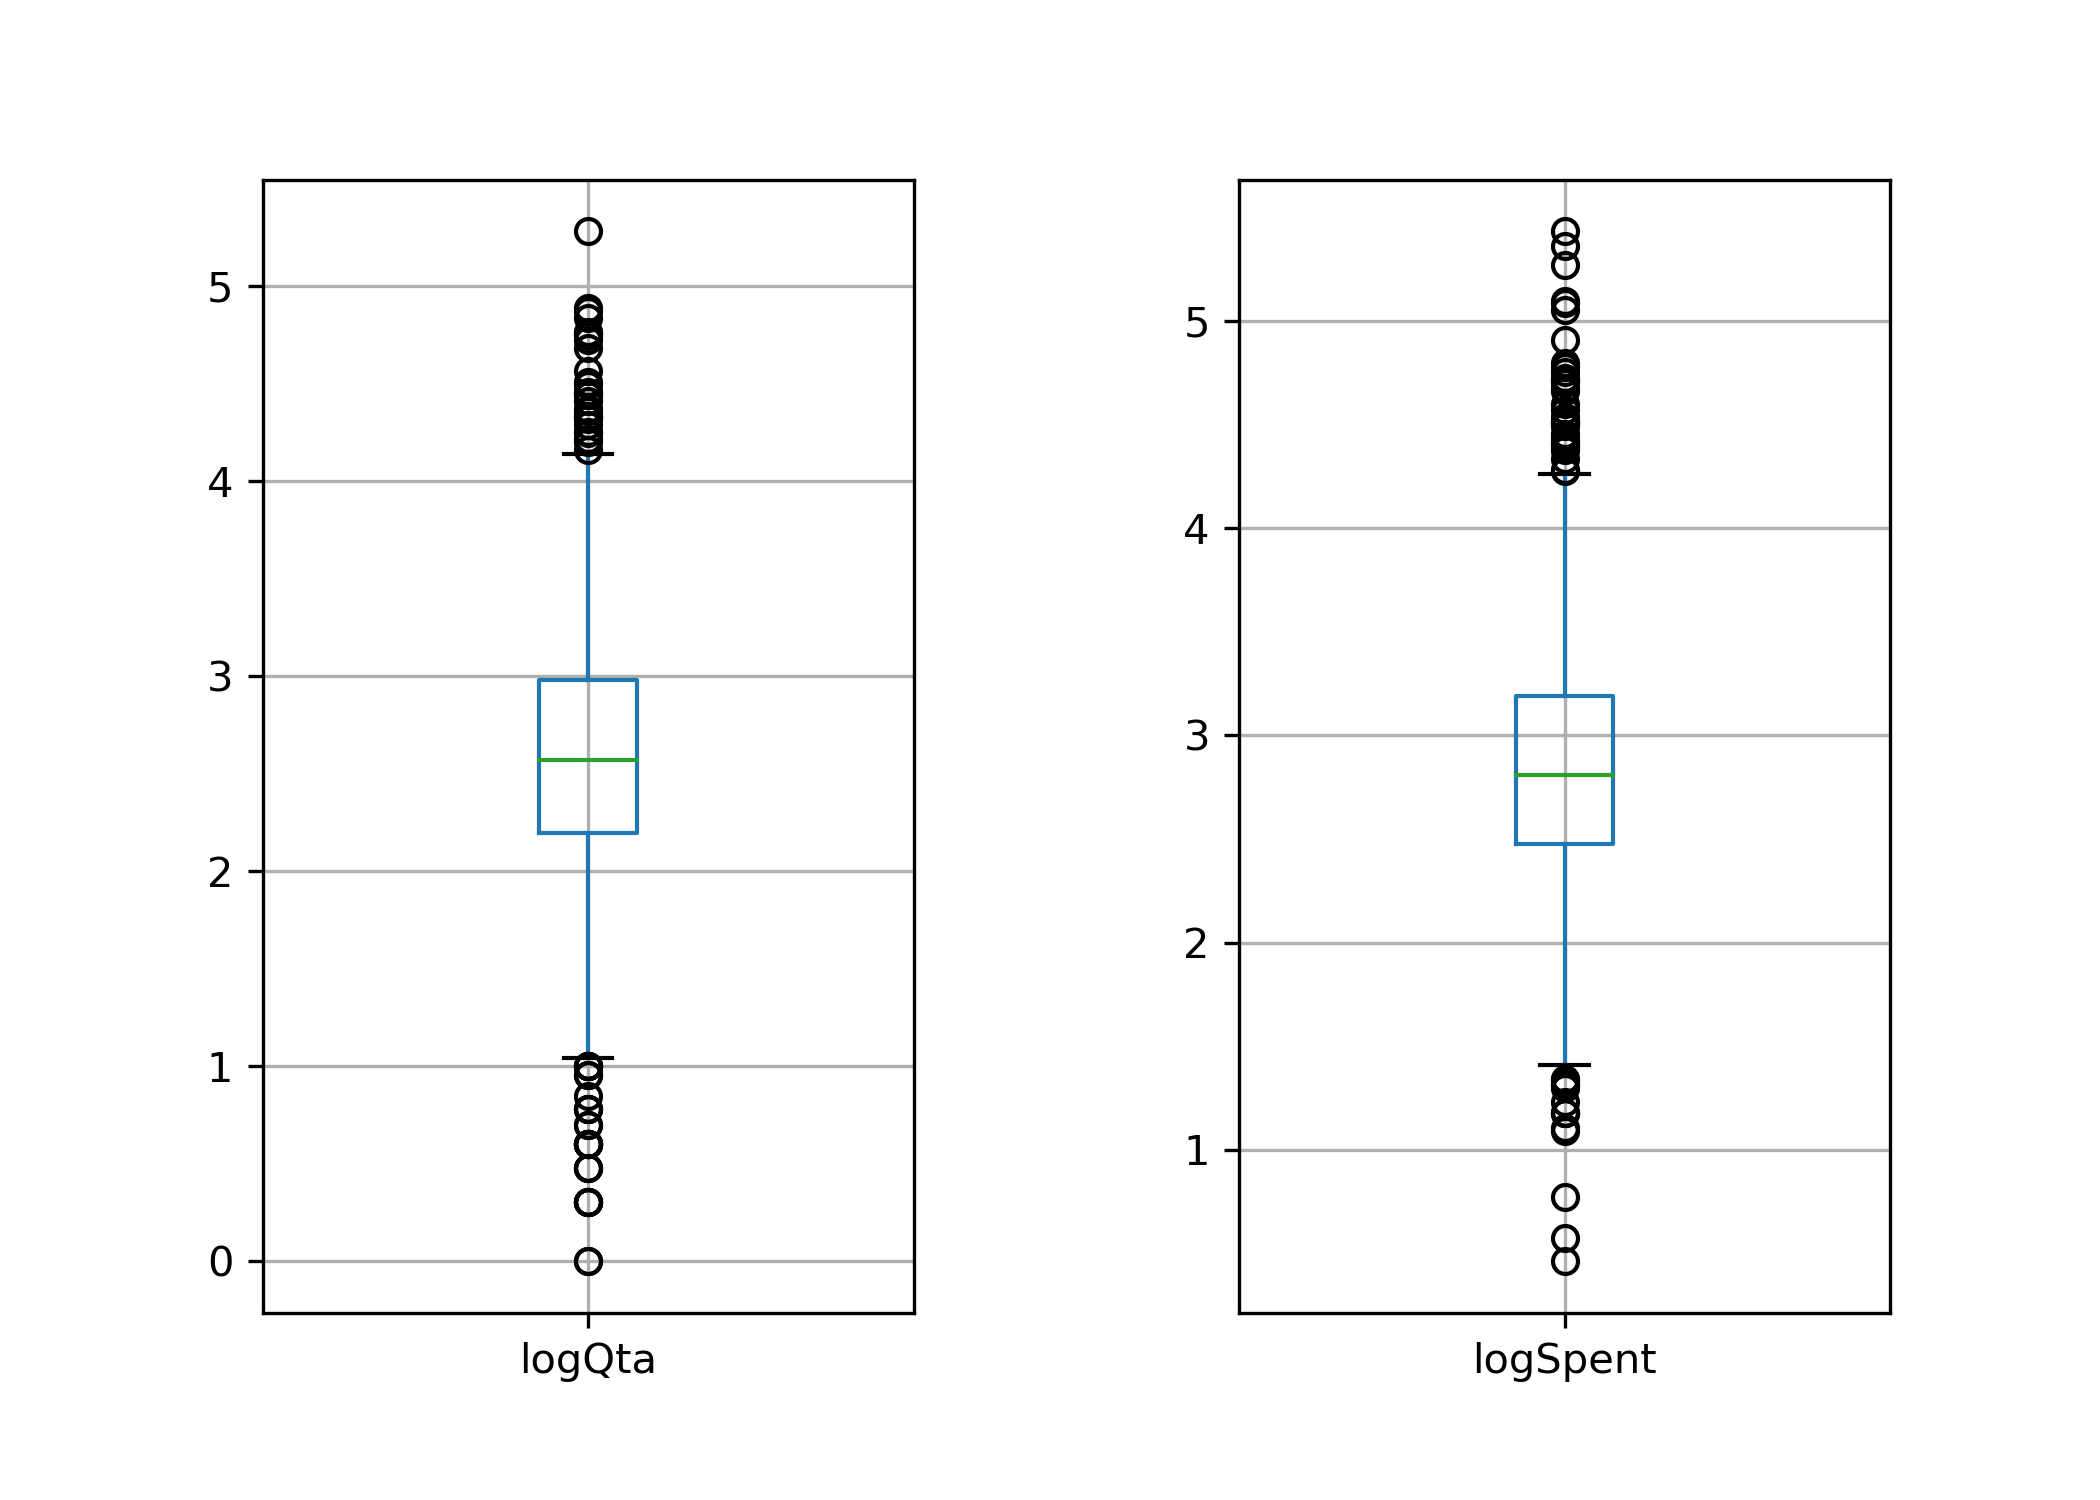
\includegraphics[width=\textwidth]{img/boxplot_for_log_actuals.png}
\caption{}
\label{fig:boxplot_logs}
\end{subfigure}
\caption{Box plots for ActualQta and ActualSpent, before and after the log}
\end{figure}

Analyzing the Figure \ref{fig:boxplot_actuals}, we can see that the attributes \textbf{ActualQta} and \textbf{ActualSpent} are really spread; for this reason, we consider their logarithm in base 10, so that the difference between high values has a different weight. We can appreciate the changes in the Figure \ref{fig:boxplot_logs}, where the two distributions are much more compact.\\
After the transformations of these attributes, we saw that also \textbf{AvgPrice} and \textbf{AvgBaskValue} were quite spread, and so we decided to compute the same operation to them.

\pagebreak

Now, we can visualize the correlation between the attributes. In Figure \ref{fig:corr_logs}, as expected, we find that the average basket value is highly correlated with the total quantity purchased and the amount of money spent. Furthermore, we can see that also the monthly frequency is correlated with the amount spent and the total quantity. In the end, of course, the quantity purchased is very highly correlated with the total amount spent.

In Figure \ref{fig:pairplot}, we can visualize the pairplot for the attributes we have.\\
On the diagonal, we have the density plots, where we can appreciate the distribution of the features. Instead, the other scatter plots show the relationship between two variables. By analyzing those, we can have a confirmation of what we already found thanks to the previous plot. 

\begin{figure}
\begin{subfigure}{.49\textwidth}
\centering
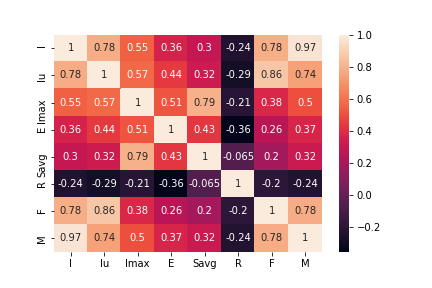
\includegraphics[width=.95\textwidth]{img/features_corr.png}
\caption{}
\label{fig:features_corr}
\end{subfigure}
\begin{subfigure}{.49\textwidth}
\centering
\captionsetup{justification=centering}
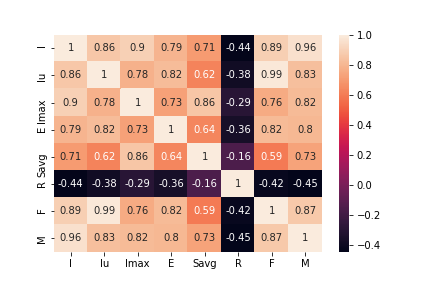
\includegraphics[width=.95\textwidth]{img/features_corr_logs.png}
\caption{}
\label{fig:features_corr_logs}
\end{subfigure}
\caption{Correlation Matrix before and after log-normalization}
\end{figure}

\begin{figure}
\begin{subfigure}{.49\textwidth}
\centering
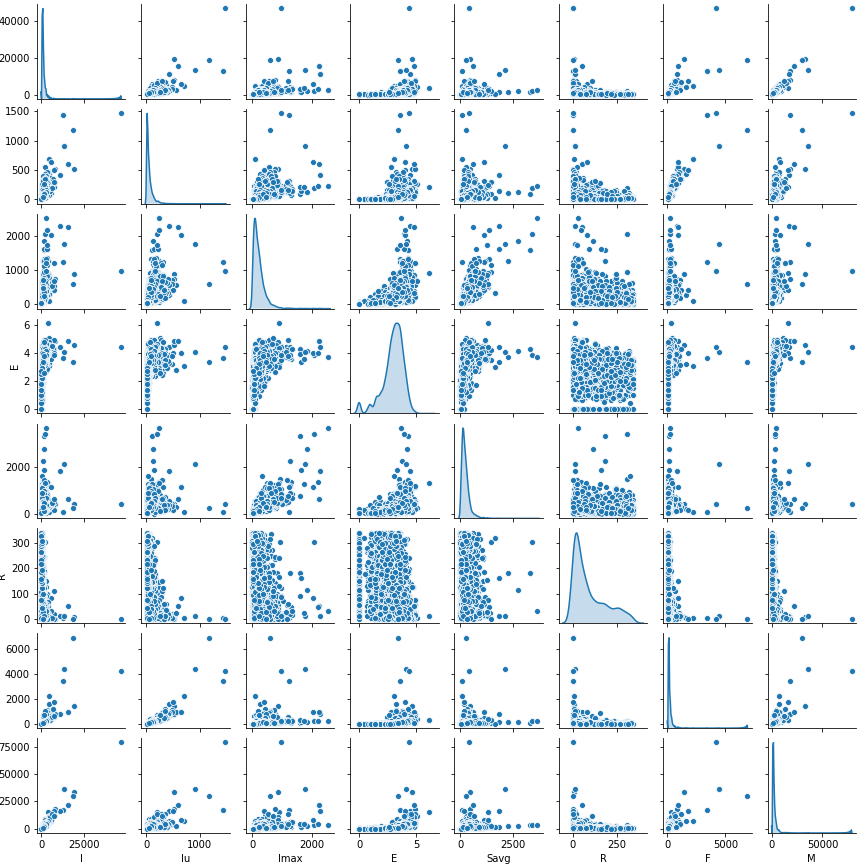
\includegraphics[width=.95\textwidth]{img/features_pairplot.png}
\caption{}
\label{fig:features_pairplot}
\end{subfigure}
\begin{subfigure}{.49\textwidth}
\centering
\captionsetup{justification=centering}
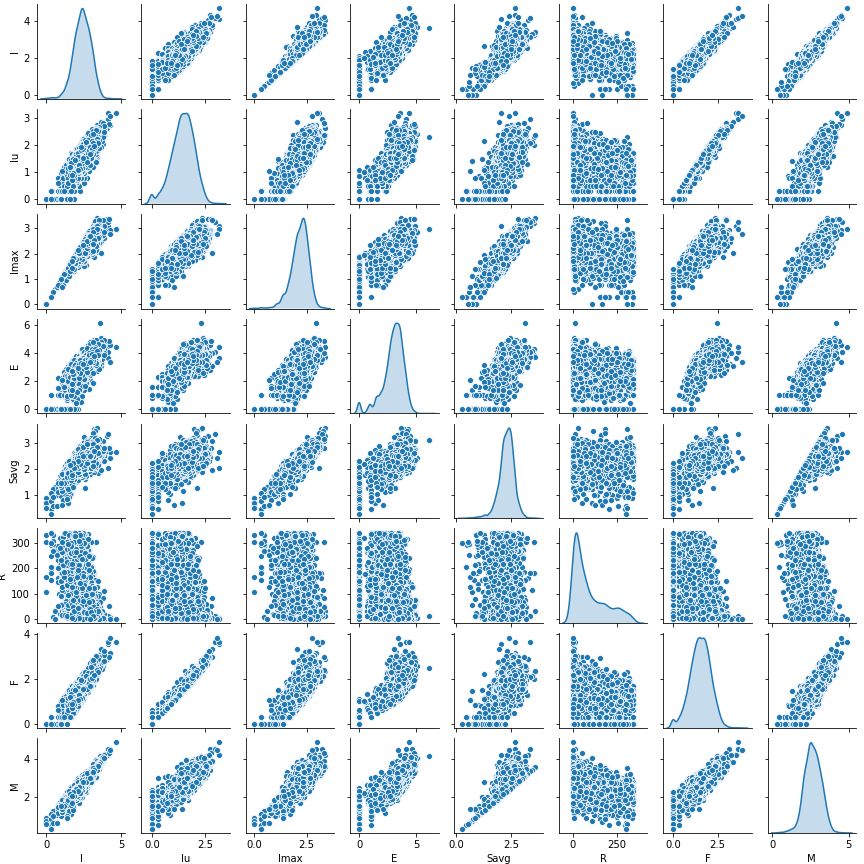
\includegraphics[width=.95\textwidth]{img/features_pairplot_logs.png}
\caption{}
\label{fig:features_pairplot_logs}
\end{subfigure}
\caption{Pairplots before and after log-normalization}
\end{figure}